\section{Casi d'uso}
\subsection{Attore}
Essendo il nostro un progetto didattico senza previsione di distribuzione, l'attore che interagisce con il nostro software è unico, denominato "Utente".\\
\textbf{Utente:} soggetto che utilizza la web application, sfruttandone le funzionalità.
\subsection{UC1 - Visualizzazione lista API disponibili}
\begin{figure}[h!]
    \centering
    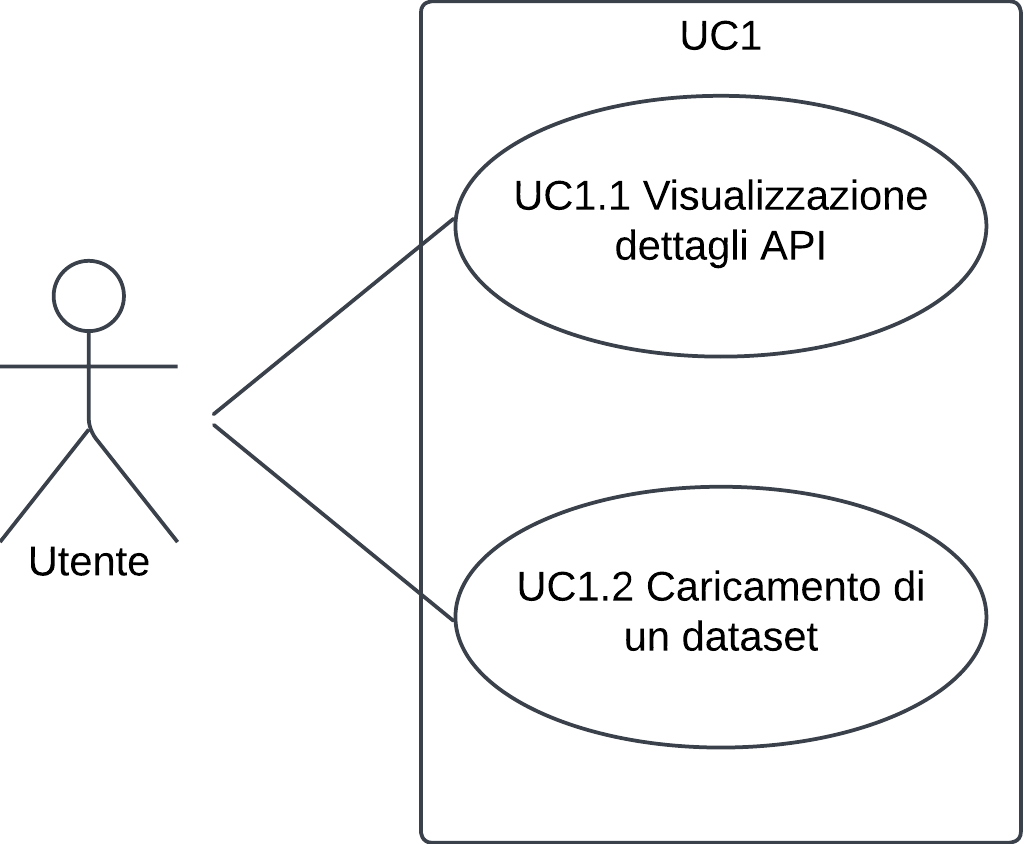
\includegraphics[scale=0.7]{template/images/UC1_1.1_1.2.png}
    \caption{UC1 - Visualizzazione lista API disponibili}
\end{figure}
\begin{itemize}
    \item \textbf{Attore:} utente;
    \item \textbf{Descrizione:} UC1 - Visualizzare la lista delle API disponibili significa che quando un utente interagisce con l'applicazione web,
    gli verrà mostrata una lista di API.\\ Da questa lista, potrà scegliere il dataset da rappresentare sotto forma di tabella e grafico 3D.
    \item \textbf{Precondizioni:}
    \begin{itemize}
        \item L'utente ha accesso all'applicazione e l'interfaccia è stata caricata correttamente;
        \item Il sistema dispone di un elenco di API disponibili da mostrare.
    \end{itemize}
    \item \textbf{Postcondizioni:}
    \begin{itemize}
        \item L'utente vede una lista delle API disponibili.
    \end{itemize}
    \item \textbf{Scenario:} 
    \begin{itemize}
        \item L'utente carica l'applicazione;
        \item Le API disponibili vengono presentate tramite un elenco;
        \item L'utente può navigare l'elenco e scegliere il dataset che gli interessa.
    \end{itemize}
\end{itemize}
\newpage
\subsubsection{UC1.1 - Visualizzazione dettagli API}
\begin{figure}[h!]
    \centering
    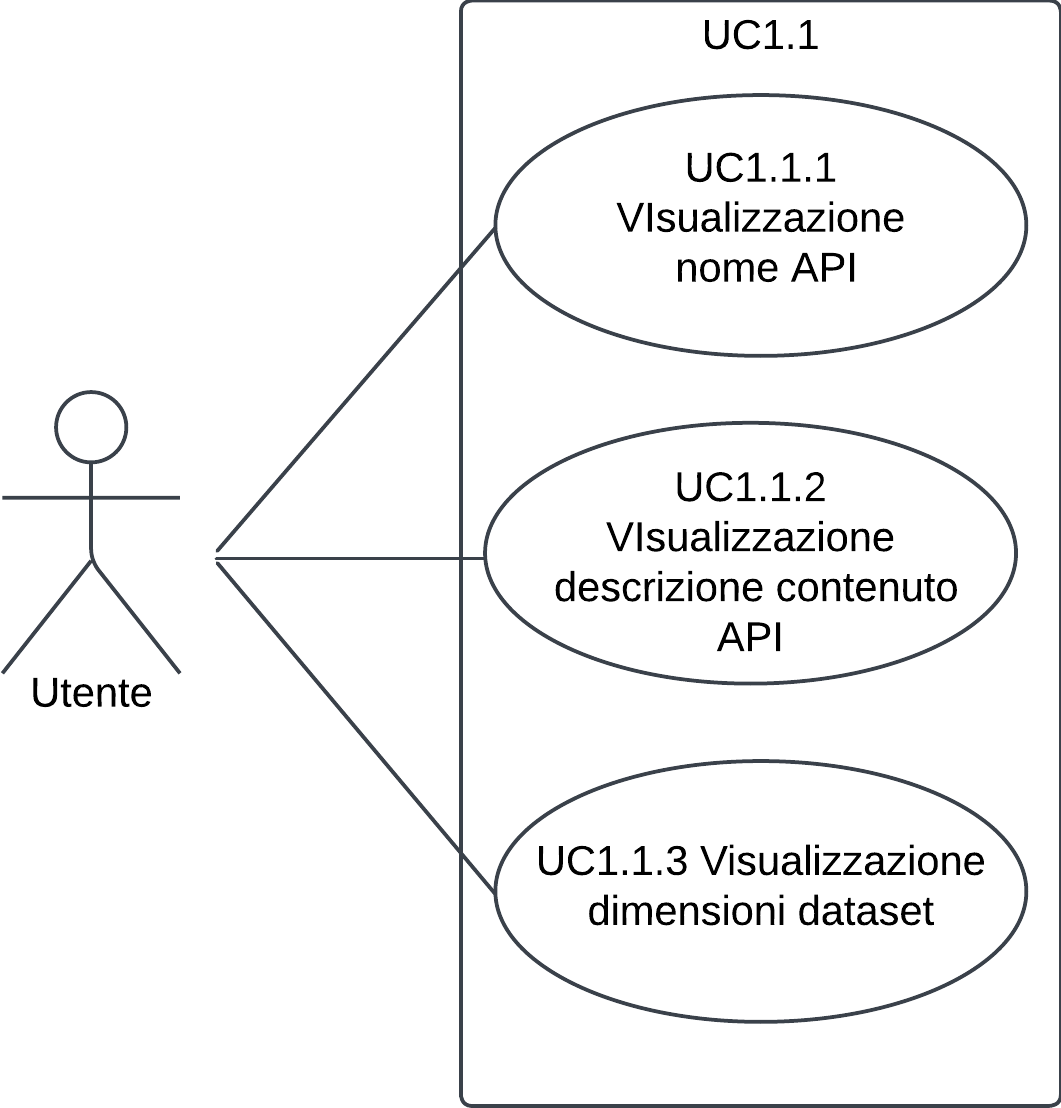
\includegraphics[scale=0.7]{template/images/UC1.1_1.1.1_1.1.2_1.1.3.png}
    \caption{UC1.1 - Visualizzazione dettagli API}
\end{figure}
\begin{itemize}
    \item \textbf{Attore:} utente;
    \item \textbf{Descrizione:} permette di visualizzare i dettagli dell'API selezionata;
    \item \textbf{Precondizioni:}
    \begin{itemize}
        \item Il sistema ha accesso ai dettagli tecnici e descrittivi delle API.
    \end{itemize}
    \item \textbf{Postcondizioni:}
    \begin{itemize}
        \item Le informazioni delle API vengono mostrate all'utente.
    \end{itemize}
    \item \textbf{Scenario:}
    \begin{itemize}
        \item L'utente seleziona un'API, e il sistema mostra i relativi dettagli.
    \end{itemize}
\end{itemize}
\paragraph{UC1.1.1 - Visualizzazione nome API}
\begin{itemize}
    \item \textbf{Attore:} Utente;
    \item \textbf{Descrizione:} L'utente può visualizzare il nome dell'API selezionata;
    \item \textbf{Precondizioni:}
    \begin{itemize}
        \item Il sistema ha accesso alle informazioni dell'API.
        \item L'utente ha selezionato un'API.
    \end{itemize}
    \item \textbf{Postcondizioni:}
    \begin{itemize}
        \item Il nome dell'API selezionata viene mostrato all'utente.
    \end{itemize}
    \item \textbf{Scenario:}
    \begin{itemize}
        \item L'utente seleziona un'API dall'interfaccia.
        \item Il sistema mostra il nome dell'API selezionata.
    \end{itemize}
\end{itemize}
\paragraph{UC1.1.2 - Visualizzazione descrizione contenuto chiamata API}
\begin{itemize}
    \item \textbf{Attore:} Utente;
    \item \textbf{Descrizione:} L'utente può visualizzare una descrizione del contenuto della chiamata all'API selezionata;
    \item \textbf{Precondizioni:}
    \begin{itemize}
        \item Il sistema ha accesso alle informazioni dell'API.
        \item L'utente ha selezionato un'API.
    \end{itemize}
    \item \textbf{Postcondizioni:}
    \begin{itemize}
        \item La descrizione del contenuto della chiamata all'API viene mostrata all'utente.
    \end{itemize}
    \item \textbf{Scenario:}
    \begin{itemize}
        \item L'utente seleziona un'API dall'interfaccia.
        \item Il sistema mostra una descrizione del contenuto della chiamata all'API.
    \end{itemize}
\end{itemize}
\paragraph{UC1.1.3 - Visualizzazione dimensioni tabella}
\begin{itemize}
    \item \textbf{Attore:} Utente;
    \item \textbf{Descrizione:} L'utente può visualizzare le dimensioni della tabella restituita dall'API selezionata;
    \item \textbf{Precondizioni:}
    \begin{itemize}
        \item Il sistema ha accesso alle informazioni dell'API.
        \item L'utente ha selezionato un'API.
    \end{itemize}
    \item \textbf{Postcondizioni:}
    \begin{itemize}
        \item Le dimensioni della tabella restituita dall'API vengono mostrate all'utente.
    \end{itemize}
    \item \textbf{Scenario:}
    \begin{itemize}
        \item L'utente seleziona un'API dall'interfaccia.
        \item Il sistema mostra le dimensioni della tabella restituita dall'API.
    \end{itemize}
\end{itemize}

\subsubsection{UC1.2 - Caricamento di un dataset dall'elenco di quelli disponibili}
\begin{itemize}
    \item \textbf{Attore:} utente;
    \item \textbf{Descrizione:} permette di caricare il dataset reperito dall'API selezionata nell'ambiente 3D dell'applicazione;
    \item \textbf{Precondizioni:}
    \begin{itemize}
        \item L'elenco dei dataset disponibili è stato caricato correttamente;
        \item L'utente seleziona un dataset dall'elenco.
    \end{itemize}
    \item \textbf{Postcondizioni:}
    \begin{itemize}
        \item Il dataset selezionato viene caricato nel sistema.
    \end{itemize}
    \item \textbf{Scenario:}
    \begin{itemize}
        \item L'utente sceglie un dataset dall'elenco disponibile;
        \item Il sistema prepara i dati per la visualizzazione in forma tabellare e in grafico 3D.
    \end{itemize}
\end{itemize}
\newpage
\subsection{UC2 - Visualizzazione dati in forma tabellare}
\begin{figure}[h!]
    \centering
    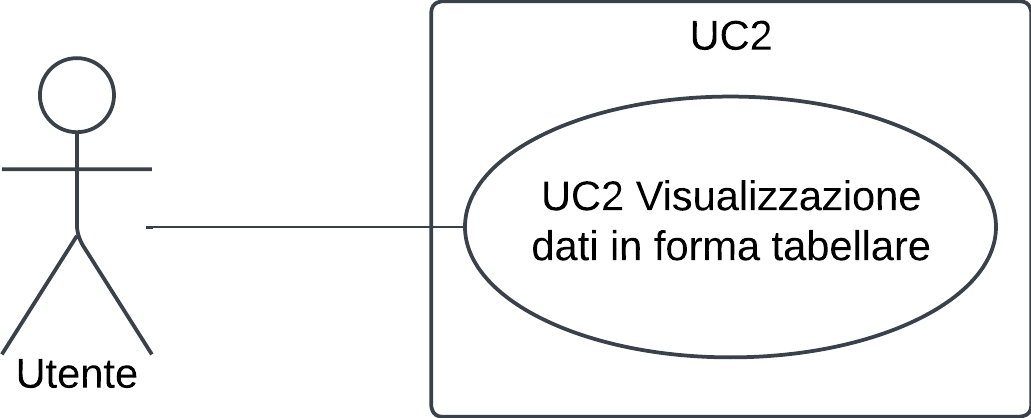
\includegraphics[scale=0.7]{template/images/UC2.png}
    \caption{UC2 - Visualizzazione dati in forma tabellare}
\end{figure}
\begin{itemize}
    \item \textbf{Attore:} utente;
    \item \textbf{Descrizione:} permette di visualizzare il dataset caricato sotto forma di tabella;
    \item \textbf{Precondizioni:}
    \begin{itemize}
        \item Un dataset è stato caricato correttamente;
        \item Il sistema è in grado di trasformare il dataset in una rappresentazione tabellare.
    \end{itemize}
    \item \textbf{Postcondizioni:}
    \begin{itemize}
        \item I dati sono mostrati in forma tabellare.
    \end{itemize}
    \item \textbf{Scenario:}
    \begin{itemize}
        \item Il dataset viene caricato correttamente;
        \item L'applicazione elabora i dati e vengono mostrati sotto forma di tabella.
    \end{itemize}
\end{itemize}
\subsection{UC3 - Visualizzazione dati in forma di grafico a istogramma 3D verticale}
\begin{figure}[h!]
    \centering
    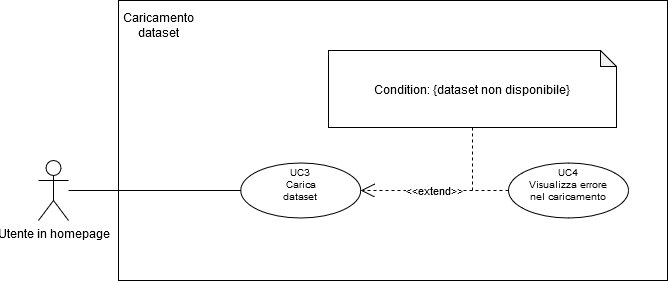
\includegraphics[scale=0.7]{template/images/UC3.png}
    \caption{UC3 - Visualizzazione dati in forma di grafico a istogramma 3D verticale}
\end{figure}
\begin{itemize}
    \item \textbf{Attore:} utente;
    \item \textbf{Descrizione:} consente di visualizzare il dataset caricato sotto forma di grafico a istogramma 3D verticale;
    \item \textbf{Precondizioni:}
    \item \begin{itemize}
        \item Un dataset è stato caricato correttamente;
        \item Il sistema è in grado di generare un grafico 3D partendo dai dati;
        \item Il sistema dispone delle informazioni necessarie per generare un grafico a istogramma.
    \end{itemize}
    \item \textbf{Postcondizioni:}
    \begin{itemize}
        \item I dati sono mostrati in forma di grafico a istogramma 3D verticale.
    \end{itemize}
    \item \textbf{Scenario:}
    \begin{itemize}
        \item Il dataset viene caricato correttamente;
        \item L'applicazione elabora i dati e viene creato un grafico a istogramma 3D verticale;
        \item L'interfaccia visualizza il grafico 3D verticale in una vista interattiva, consentendo all'utente di analizzare i dati.
    \end{itemize}
\end{itemize}
\subsection{UC4 - Visualizzazione assi}
\begin{figure}[h!]
    \centering
    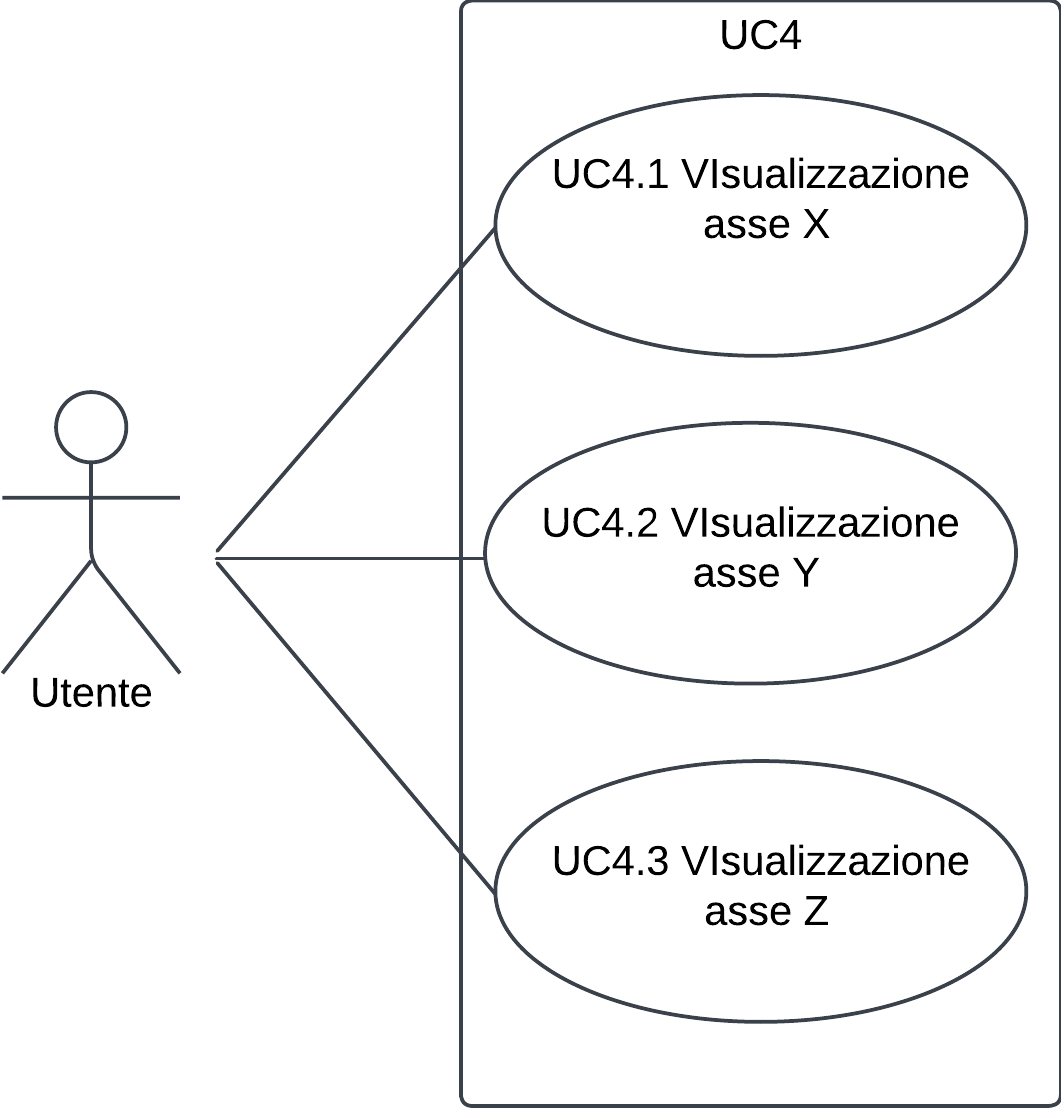
\includegraphics[scale=0.7]{template/images/UC4.png}
    \caption{UC4 - Visualizzazione assi}
\end{figure}
\begin{itemize}
    \item \textbf{Attore:} utente;
    \item \textbf{Descrizione:} permette di visualizzare dettagliatamente le assi X, Y e Z del grafico;
    \item \textbf{Precondizioni:} 
    \item \begin{itemize}
        \item Il grafico 3D è stato generato correttamente;
        \item Gli assi sono configurati nel sistema.
    \end{itemize}
    \item \textbf{Postcondizioni:}
    \begin{itemize}
        \item Gli assi X, Y e Z sono visibili e ben etichettati.
    \end{itemize}
    \item \textbf{Scenario:} nessuno.
\end{itemize}
\subsubsection{UC4.1 - Visualizzazione asse X}
\begin{itemize}
    \item \textbf{Attore:} utente;
    \item \textbf{Descrizione:} permette di visualizzare dettagliatamente l'asse X;
    \item \textbf{Precondizioni:} 
    \item \begin{itemize}
        \item L'asse X è configurato nel grafico.
    \end{itemize}
    \item \textbf{Postcondizioni:} 
    \begin{itemize}
        \item L'asse X è visibile e mostra i valori appropriati.
    \end{itemize}
    \item \textbf{Scenario:} nessuno.
\end{itemize}
\subsubsection{UC4.2 - Visualizzazione asse Y}
\begin{itemize}
    \item \textbf{Attore:} utente;
    \item \textbf{Descrizione:} permette di visualizzare dettagliatamente l'asse Y;
    \item \textbf{Precondizioni:} 
    \item \begin{itemize}
        \item L'asse Y è configurato nel grafico.
    \end{itemize}
    \item \textbf{Postcondizioni:} 
    \begin{itemize}
        \item L'asse Y è visibile e mostra i valori appropriati.
    \end{itemize}
    \item \textbf{Scenario:} nessuno.
\end{itemize}
\subsubsection{UC4.3 - Visualizzazione asse Z}
\begin{itemize}
    \item \textbf{Attore:} utente;
    \item \textbf{Descrizione:} permette di visualizzare dettagliatamente l'asse Z;
    \item \textbf{Precondizioni:} 
    \item \begin{itemize}
        \item L'asse Z è configurato nel grafico.
    \end{itemize}
    \item \textbf{Postcondizioni:} 
    \begin{itemize}
        \item L'asse Z è visibile e mostra i valori appropriati.
    \end{itemize}
    \item \textbf{Scenario:} nessuno.
\end{itemize}
\subsection{UC5 - Visualizzazione legenda}
\begin{figure}[h!]
    \centering
    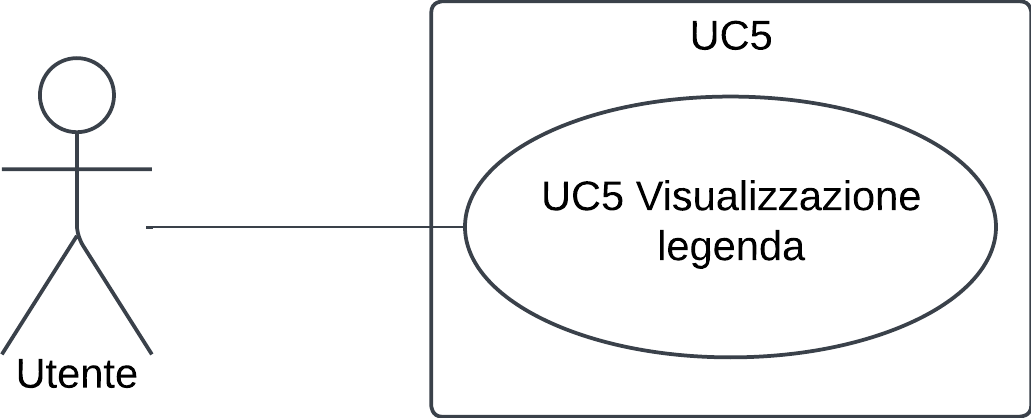
\includegraphics[scale=0.7]{template/images/UC5.png}
    \caption{UC5 - Visualizzazione legenda}
\end{figure}
\begin{itemize}
    \item \textbf{Attore:} utente;
    \item \textbf{Descrizione:} permette di visualizzare una legenda, contenente dettagli e informazioni sul grafico;
    \item \textbf{Precondizioni:} 
    \begin{itemize}
        \item Il grafico 3D è stato generato correttamente;
        \item Il sistema dispone delle informazioni necessarie per creare una legenda.
    \end{itemize}
    \item \textbf{Postcondizioni:}
    \begin{itemize}
        \item La legenda è visibile e fornisce informazioni dettagliate che aiutano l'utente a comprendere i dati rappresentati.
    \end{itemize}
    \item \textbf{Scenario:} nessuno.
\end{itemize}
\newpage
\subsection{UC6 - Pan}
\begin{figure}[h!]
    \centering
    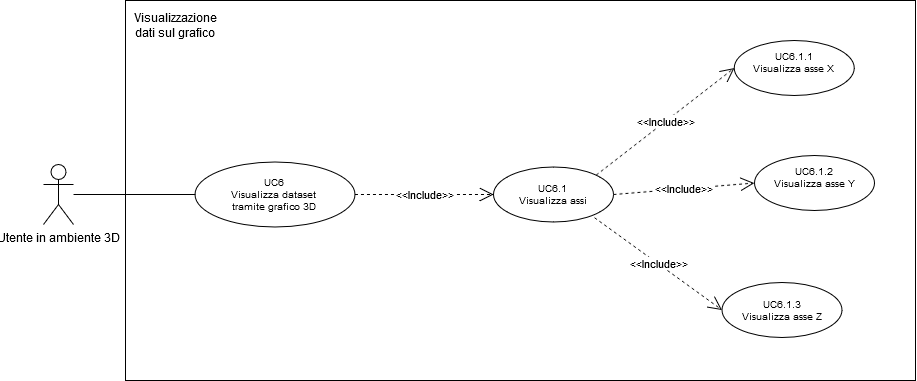
\includegraphics[scale=0.7]{template/images/UC6.png}
    \caption{UC6 - Funzionalità PAN}
\end{figure}
\begin{itemize}
    \item \textbf{Attore:} utente;
    \item \textbf{Descrizione:} l'utente desidera spostare la visualizzazione del grafico 3D lungo il piano XY senza modificare l'orientamento della camera;
    \item \textbf{Precondizioni:}
    \begin{itemize}
        \item L'utente sta visualizzando il grafico 3D;
        \item Il sistema ha abilitato la funzionalità di interazione pan.
    \end{itemize}
    \item \textbf{Postcondizioni}:
    \begin{itemize}
        \item La vista della scena 3D è stata spostata nella direzione indicata dall'utente.
    \end{itemize}
    \item \textbf{Scenario:}
    \begin{itemize}
        \item L'utente visualizza il grafico 3D nell'interfaccia;
        \item L'utente interagisce con il grafico utilizzando il mouse (trascinamento);
        \item Il sistema interpreta il comando di spostamento e aggiorna la posizione del grafico lungo il piano XY;
        \item La nuova vista viene aggiornata in tempo reale e mostrata all'utente.
    \end{itemize}
\end{itemize}
\subsection{UC7 - Rotazione camera}
\begin{figure}[h!]
    \centering
    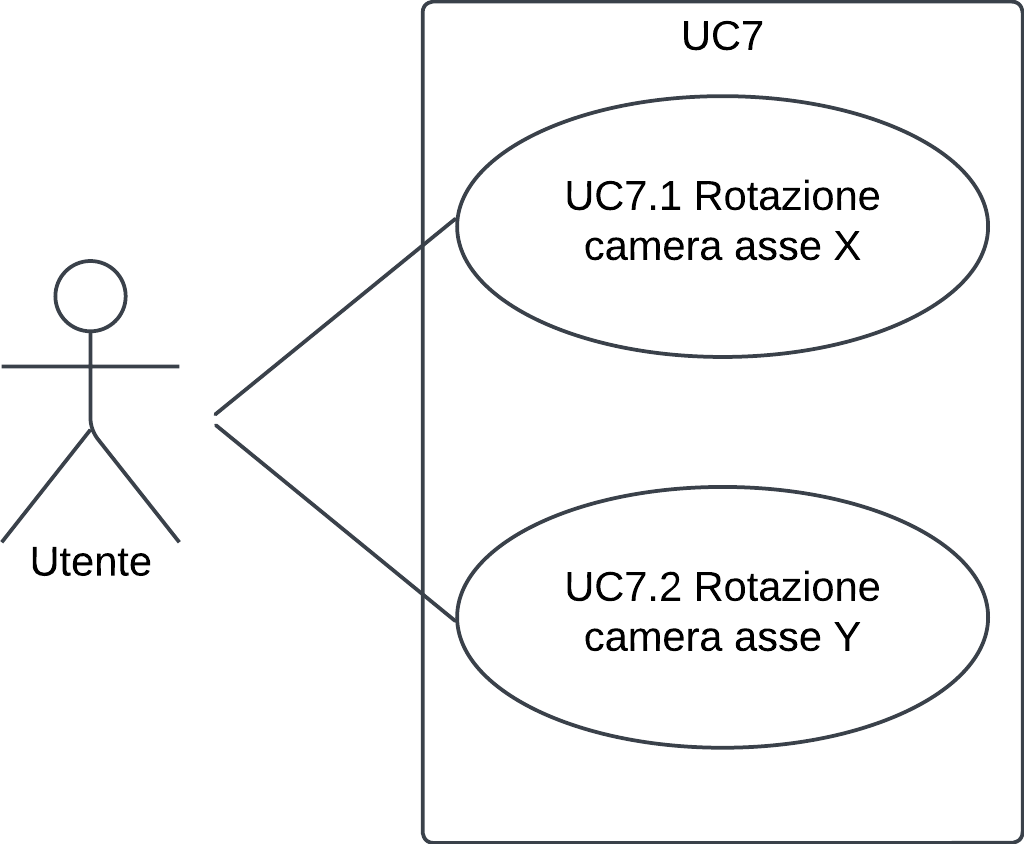
\includegraphics[scale=0.7]{template/images/UC7_7.1_7.2.png}
    \caption{UC7 - Rotazione camera}
\end{figure}
\begin{itemize}
    \item \textbf{Attore:} utente;
    \item \textbf{Descrizione:} l'utente desidera ruotare la visualizzazione del grafico 3D modificando l'orientamento della camera lungo uno o più assi. La rotazione consente di analizzare il grafico da diverse angolazioni;
    \item \textbf{Precondizioni:} 
    \begin{itemize}
        \item L'utente sta visualizzando il grafico 3D nell'interfaccia;
        \item Il sistema ha abilitato le funzionalità di interazione con la camera.
    \end{itemize}
    \item \textbf{Postcondizioni:} 
    \begin{itemize}
        \item La visualizzazione del grafico è stata aggiornata in base alla rotazione effettuata dall'utente.
    \end{itemize}
    \item \textbf{Scenario:}  
    L'utente interagisce con il grafico 3D usando i comandi per ruotare la visualizzazione. Il sistema aggiorna in tempo reale l'orientamento della camera, mostrando il grafico da una nuova angolazione.
\end{itemize}
\subsubsection{UC7.1 - Rotazione camera asse X}
\begin{itemize}
    \item \textbf{Attore:} utente;
    \item \textbf{Descrizione:} l'utente ruota la visualizzazione del grafico 3D attorno all'asse X, modificando l'altezza della prospettiva.
    \item \textbf{Precondizioni:} 
    \begin{itemize}
        \item L'utente sta visualizzando il grafico 3D nell'interfaccia;
        \item Il sistema ha abilitato le funzionalità di interazione con la camera.
    \end{itemize}
    \item \textbf{Postcondizioni:} 
    \begin{itemize}
        \item La camera è stata ruotata attorno all'asse X, aggiornando la vista in tempo reale.
    \end{itemize}
    \item \textbf{Scenario:}  
    L'utente usa comandi per spostare la vista verso l'alto o verso il basso. Il sistema ruota la camera attorno all'asse X, consentendo di osservare il grafico da un'angolazione più alta o più bassa.
\end{itemize}
\subsubsection{UC7.2 - Rotazione camera asse Y}
\begin{itemize}
    \item \textbf{Attore:} utente;
    \item \textbf{Descrizione:} L'utente ruota la visualizzazione del grafico 3D attorno all'asse Y, modificando l'orientamento laterale della prospettiva;
    \item \textbf{Precondizioni:} 
    \begin{itemize}
        \item L'utente sta visualizzando il grafico 3D nell'interfaccia;
        \item Il sistema ha abilitato le funzionalità di interazione con la camera.
    \end{itemize}
    \item \textbf{Postcondizioni:} 
    \begin{itemize}
        \item La camera è stata ruotata attorno all'asse Y, aggiornando la vista in tempo reale.
    \end{itemize}
    \item \textbf{Scenario:}  
    L'utente usa comandi per spostare la vista verso destra o sinistra. Il sistema ruota la camera attorno all'asse Y, consentendo di osservare il grafico da angolazioni diverse lateralmente.
\end{itemize}


